\chapter{Firm-size distribution}
\label{app:size-distribution}

Figure~\ref{fig:size-distribution} measures the stationary distribution of relative sizes
$S_i=Nw_i$ at the operating point: ten independent $N=10000$ economies, each observed over the
late window $t\in[180,240]$. The left panel keeps every observation; its lower plateau is set by the
immigration floor. The reporting cut $S=0.1$, applied only in the upper-tail panel, removes this
floor-dominated region and is not a graph cutoff. On log--log axes the active-firm tail bends
sharply instead of following a straight Pareto segment. A fit of the complementary-tail exponent
in each economy, from its upper $2\%$ of active observations, gives $\hat\mu=4.40$ with a $95\%$
$t$ interval $[4.02,4.78]$; a Zipf tail has exponent near one. The upper tail at this operating
point is far thinner, effectively truncated.

The main results of the thesis are therefore claims about the size-conditioned growth
fluctuations and their network origin, not about the cross-sectional size distribution,
which the model at this operating point does not reproduce.

\begin{figure}[!htb]
    \centering
    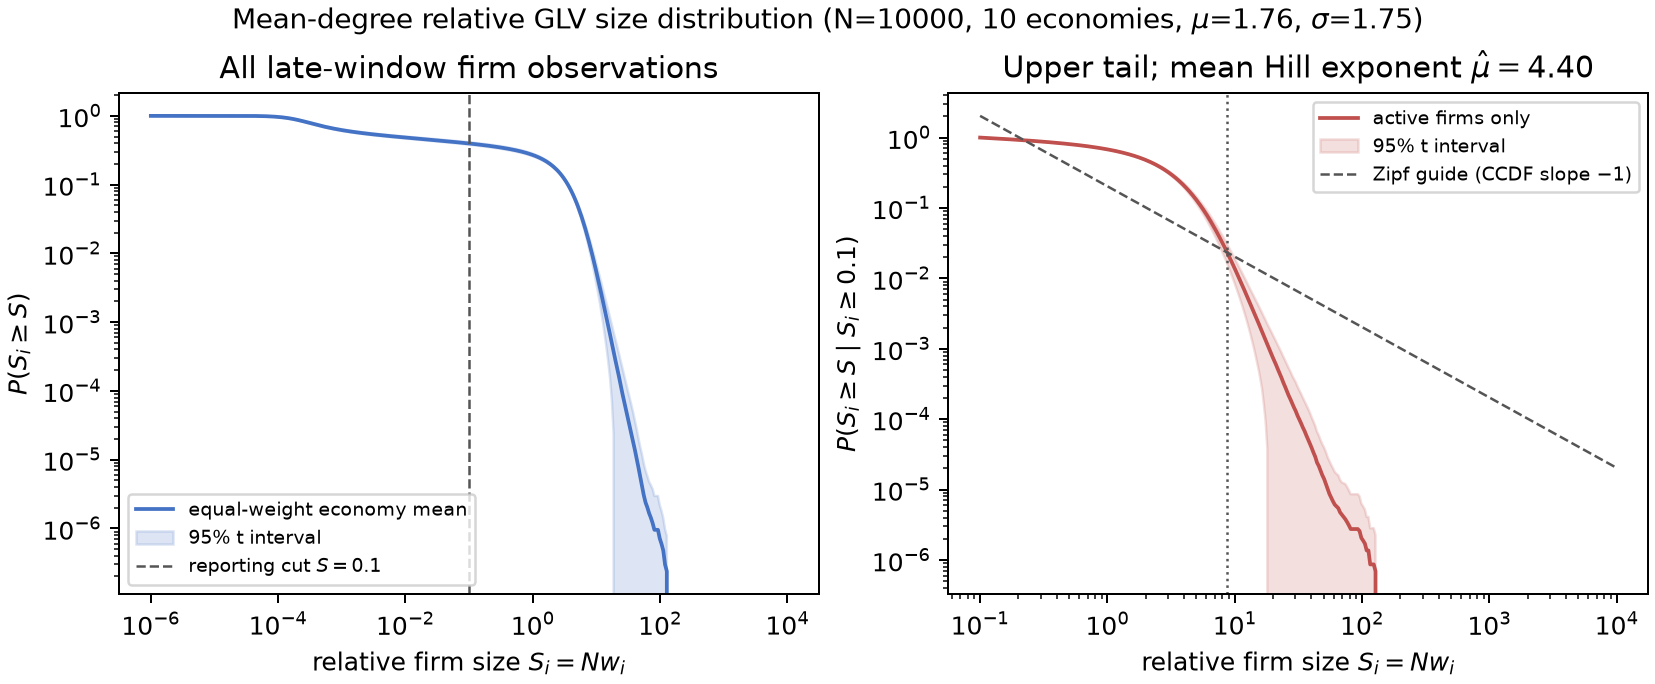
\includegraphics[width=0.82\linewidth]{size_distribution_N10000.png}
    \caption{Stationary relative firm-size distribution in the mean-degree power-law
    ensemble ($N=10000$, $C=250$, ten economies, $\mu=-1.76$, $\sigma=1.75$). Curves are
    equal-weight means of economy-level complementary distribution functions; shading is the
    $95\%$ interval across economies. \panel{Left}: all late-window observations.
    \panel{Right}: conditional upper tail of active firms, with strong curvature and a
    complementary-tail exponent near $4.4$ against the Zipf benchmark near $1$.}
    \label{fig:size-distribution}
\end{figure}
